\documentclass[conference,compsoc]{IEEEtran}

\ifCLASSOPTIONcompsoc
  \usepackage[nocompress]{cite}
\else
  % normal IEEE
  \usepackage{cite}
  \usepackage{graphicx}
  \usepackage{graphicx}
  \usepackage{url}
  \usepackage[english]{babel}
  \usepackage{times}
  \usepackage{amssymb}
  \usepackage{color}
  \usepackage{xspace}
  \usepackage{listings}
  \usepackage{upquote}
  \usepackage{amsmath}
  \usepackage[hidelinks]{hyperref}
  \usepackage{wrapfig}
  \graphicspath{ {/Users/tejasK/Documents/ASU Coursework/FSL/Project/IEEEtran/} }
\fi

\ifCLASSINFOpdf
  \usepackage[pdftex]{graphicx}
   \usepackage{url}
  \usepackage[english]{babel}
  \usepackage{times}
  \usepackage{amssymb}
  \usepackage{color}
  \usepackage{xspace}
  \usepackage{listings}
  \usepackage{upquote}
  \usepackage[hidelinks]{hyperref}
  \usepackage{wrapfig}
  \graphicspath{ {/Users/tejasK/Documents/ASU Coursework/FSL/Project/IEEEtran/} }

\else

  \usepackage[dvips]{graphicx}
   \usepackage{url}
  \usepackage[english]{babel}
  \usepackage{times}
  \usepackage{amssymb}
  \usepackage{color}
  \usepackage{xspace}
  \usepackage{listings}
  \usepackage{upquote}
  \usepackage[hidelinks]{hyperref}
  \usepackage{wrapfig}
  \graphicspath{ {/Users/tejasK/Documents/ASU Coursework/FSL/Project/IEEEtran/} }
\fi

\hyphenation{op-tical net-works semi-conduc-tor}


\begin{document}

\title{Multiple Instance Learning using EMDD}

\author{\IEEEauthorblockN{Tejas Khairnar}
\IEEEauthorblockA{Arizona State University\\
Email: tkhairna@asu.edu}
\and
\IEEEauthorblockN{Vivin Paliath}
\IEEEauthorblockA{Arizona State University\\
Email: tkhairna@asu.edu}}

\maketitle

\begin{abstract}
This midterm report details our understanding, approach, and progress in implementing the Estimation Maximization Diverse Density (EMDD)\cite{zhang2001dd} algorithm. EMDD is an approach that has seen success in Multiple-Instances Learning problems and is a generalization of the supervised-learning classification-problem. Our goal is to demonstrate an understanding of this algorithm by providing a valid implementation and demonstrating its performance against the supplied data sets.
\end{abstract}


\IEEEpeerreviewmaketitle


\section{Introduction}
% no \IEEEPARstart
The Multiple Instances Learning (MIL) problem is a variation of the general supervised-learning classification-problem. In MIL, instead of presenting a single instance, a bag of instances is presented to the algorithm, along with a label that describes the bag as either positive or negative. A bag is given a positive label if it contains at least one positive instance, and a negative label if it does not contain any positive instances. The goal of the MIL problem then, is to classify unseen bags or instances as either positive or negative, based on the training data. For this project, we specifically focus on the EMDD algorithm and use it to solve the MIL problem. 

\section{EMDD}

Before looking at the EMDD algorithm, it is useful to look at diverse density itself. If we assume that there is a hypothetical point $t$ in the feature space that identifies the "true concept", the goal of DD is to identify the region that has positive instances from the most number of \textit{different} positive bags, while also being far away from negative instances. Hence the diverse-density problem involves maximizing the probability $P(x = t \mid B_1^+, \dots, B_n^+, B_1^-, \dots, B_m^-)$, where $B_i^+$ is a positive bag and $B_j^-$ is a negative bag. This is effectively equivalent to maximizing the following\cite{zhang2001dd}:

\begin{equation}
\arg\max_x \prod_i P(x = t \mid B_i^+) \prod_i P(x = t \mid B_i^-)
\end{equation}

From this general definition of the maximum diverse-density, a noisy-or model is used to define the terms in the products. Hence the probability all points did not miss the target is $P(x = t \mid B_i^+) = P(x = t \mid B^+_{i1}, B^+_{i2}, \dots) = 1 - \prod_j(1 - P(x =t \mid B^+_{ij}))$ and likewise $P(x = t \mid B_i^-) = \prod_j(1 - P(x = t \mid B_{ij}^-))$. The probability of a particular instance being the potential target-instance is then based on the distance between them: $P(x = t \mid B_{ij}) = \exp(- \left\| B_{ij} - x \right\|^2)$. The intuition is that if one of the instances in a positive bag is close to $x$, then $P(x = t \mid B_i^+)$ is high. Hence, if all positive bags have an instance close to $x$ and no negative ones do, the diverse density of $x$ will be high. Also observe that while the diverse density at the intersection of $n$ bags is exponentially higher than at $n - 1$ bags, the presence of a single negative instance is enough to drive down the diverse density.

The diverse density formulation also takes into account the relevance of features learning a scaling vector $s$ in addition to the location $x$ that maximizes the diverse density ($\left\| B_{ij} - x \right\|^2 = \sum_k s_k^2(B_{ijk} - x_k)^2$). This allows the algorithm to disregard irrelevant features and consider important ones, especially considering that it uses the Euclidean distance as a metric for "closeness". 

\subsection{Diverse Density Algorithm}
The main idea of DD approach is to find a concept point in the feature space that are close to at-least one instance from every positive bag and meanwhile far away from instances in negative bags~\cite{MILlink}. The optimal concept point is defined as the one with maximum density, which is a measure of how many different positive bags have instances near the point, and how far the negative instances are from that point.
\subsection{Estimation Maximization}
The Estimation Maximization algorithm is an effective iterative procedure to compute the Maximum Likelihood (ML) estimate in the presence of missing or hidden data~\cite{EMlink}. In ML estimation, we wish to estimate the model parameter(s) for which the observed data are the most likely.
Each iteration of the EM algorithm consists of two processes: The E-step, and the M-step. In the expectation, or E-step, the missing data are estimated given the observed data and current estimate of the model parameters. This is achieved using the conditional expectation, explaining the choice of terminology. In the M-step, the likelihood function is maximized under the assumption that the missing data are known. The estimate of missing data from the E-step are used in lieu of the actual missing data.
Convergence is assured since the algorithm is guaranteed to increase the likelihood at each iteration.
\subsection{EMDD}
EM-DD~\cite{MILlink} starts with an initial guess of the concept point t (which can be obtained using original DD algorithm), and then repeatedly performs the following two steps: E-step, the current hypothesis of concept t I used to pick the most likely instances from each bag given a generative model; in M-step, a new concept t’ is estimated by maximizing a transformed DD defined on the instances selected in the E-step using the gradient search. Then, the old concept t is replaced by the new concept t’ and the two steps are repeated until the algorithm converges. This EM-DD algorithm which we have implemented, implementes a “hard” version of EM, since only one instance per bag is used for estimating the hypothsis. It can be also regarded as a special case of the K-means clustering algorithm~\cite{Harti} , where only on cluster is considered.

\section{Progress}
Until midterm, we have successfully implemented the EMDD algorithm in python programming language. In order to perform the Math behind the algorithm we are using the SciPy library~\cite{Scipy}. According to the goals allocated for this project, we have tested our implementation against the Synthetic data set~\cite{SynthDataset}. In order to perform the comparison of results obtained by our implementation and the Matlab implementation of MIL algorithms ~\cite{MILlink}, we performed the Matlab setup and ran the Matalb setup for algorithms like 
\begin{itemize}
	\item Iterated-discrim APR
	\item Diverse Density
	\item Two SVM variants for MIL
	\item Citation-kNN for MIL
\end{itemize}
Currently we have the results for these algorithms against the Synthetic dataset. We are now in progress of moving toward the public dataset list ~\cite{MILlink,andrews2002support,Lichman:2013}.

\section{Timeline}
Below is the timeline for this project which we chalked out:
\begin{figure}[t]
	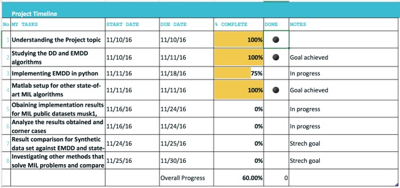
\includegraphics{timeline}
\end{figure}


\section{Results}
We don not need to put in results for our midterm report.

\section{Workload Shared}
The workload amongst us was shared equally. We worked together on the implementation. The major part of coding was done by Vivin and I took care of the Matlab setup and result comparison part. 


\section{Conclusion}
Till midterm we have successfully completed the task mentioned. We are focusing on achieving all the goals mentioned in the timeline.



% conference papers do not normally have an appendix



% use section* for acknowledgment
\ifCLASSOPTIONcompsoc
  % The Computer Society usually uses the plural form
  \section*{Acknowledgments}
\else
  % regular IEEE prefers the singular form
  \section*{Acknowledgment}
\fi


The authors would like to thank...

\bibliographystyle{abbrvnat}
\bibliography{main}{}

\end{document}


